%----------------------------------------------------------------------------------------
%	SOLUTION 2.i
%----------------------------------------------------------------------------------------
\subsection*{Solution 2.i}
\paragraph{Summary:} In case of Random forest, we randomly choose $m$ features out of $d\geq m$ features, to use for classification for each stump and learn an ensemble of $B$ stump. In each iteration, we bootstrap a sample $Z^*$ of size $N$ from the training set of size $N$ and use this data to train the stump. In this way, we train an ensemble of trees, $\{T_b\}_{b=1}^{B}$. Let, $\hat{C}_b(x)$ be the class prediction of the $b^{th}$ tree in the random forest for the sample $x$. Then the prediction of the random forest for sample $x$ is
\begin{align*}
	\hat{C}_{rf}(x) = majority\ vote\ \{\hat{C}_b(x)\}_{1}^{B}.
\end{align*}
In this homework, we are required to choose $B=100$ and for part (i) $m=3$.
\paragraph{Results:}Fig.~\ref{fig:q2i_error_rate} shows the error rate on training and test set, with $m=3$, as we increase the number of stumps in the random forest algorithm. It can be seen that as the number of trees increases both training and test error decreases while after a certain number of trees, the improvement of error rate on both training and test set become minimal.
%%%%%%%%%%%%%%%%%%%%%%% RF ERROR: M = 3 %%%%%%%%%%%%%%%%%%%%%
\begin{figure}[!h]
	\centering
	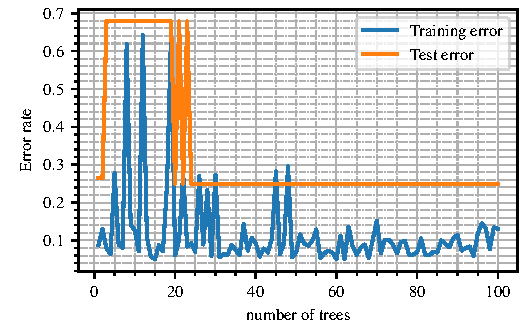
\includegraphics[scale=1.0,trim={0cm 0cm 0cm 0cm},clip]{./code/generatedPlots/q2i_error_rate.pdf}
	\caption{Q2.i: Random Forest with $m=3$: Training and test error decreases as number of trees increases}
	\label{fig:q2i_error_rate}
\end{figure}
%----------------------------------------------------------------------------------------
%	SOLUTION 2.ii
%----------------------------------------------------------------------------------------
\subsection*{Solution 2.ii}
\paragraph{Summary:} In this part we are required to plot the training and test error as we increase $m$, the number of randomly selected features to use for classification for each stump in the forest. 
\paragraph{Results:} Fig.~\ref{fig:q2ii_error_rate} shows the plot of training and test error as we increase $m$. It can be seen that both training and test error decrease with increase in $m$, however, when $m$ approaches $d$, total number of features, the error sometimes increases due to increased variance of the tree output. As, we bootstrap the training sample set before learning, each tree is trained on different sample sets which produces poor generalization accuracy if $m$ is equal to $d$. 
%%%%%%%%%%%%%%%%%%%%%%% RF ERROR VS. M %%%%%%%%%%%%%%%%%%%%%
\begin{figure}[!h]
	\centering
	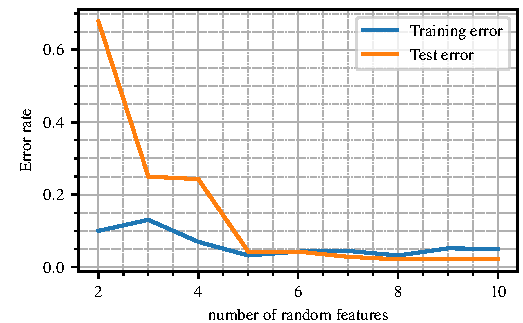
\includegraphics[scale=1.0,trim={0cm 0cm 0cm 0cm},clip]{./code/generatedPlots/q2ii_error_rate.pdf}
	\caption{Q2.ii: Random Forest with varying $m$: Training and test error}
	\label{fig:q2ii_error_rate}
\end{figure}
Fig.~\ref{fig:q2ii_error_rate_trn} shows the training error rates for different values of $m$ as we increase the number of trees. It can be seen that increasing $m$, in general decreases the error rate of random forest algorithm. The figure reveals that for any particular number of trees, increasing $m$ decreases the training error. 
%%%%%%%%%%%%%%%%%%%%%%% RF ERROR VS. M %%%%%%%%%%%%%%%%%%%%%
\begin{figure}[!h]
	\centering
	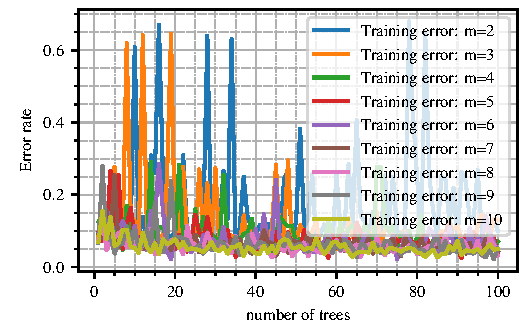
\includegraphics[scale=1.0,trim={0cm 0cm 0cm 0cm},clip]{./code/generatedPlots/q2ii_error_rate_trn.pdf}
	\caption{Q2.ii: Random Forest with varying $m$: Training error}
	\label{fig:q2ii_error_rate_trn}
\end{figure}
Fig.~\ref{fig:q2ii_error_rate_tst} shows the test error rates for different values of $m$ as we increase the number of trees. Similar trend, as we have seen in case of training error, can be seen for test error also.
%%%%%%%%%%%%%%%%%%%%%%% RF ERROR VS. M %%%%%%%%%%%%%%%%%%%%%
\begin{figure}[!h]
	\centering
	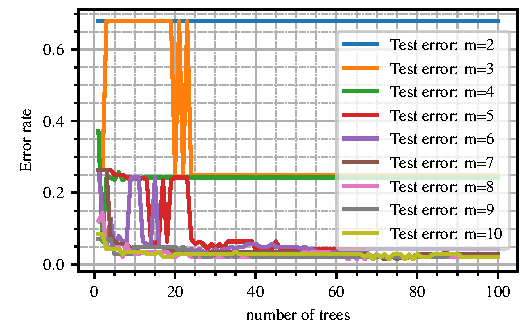
\includegraphics[scale=1.0,trim={0cm 0cm 0cm 0cm},clip]{./code/generatedPlots/q2ii_error_rate_tst.pdf}
	\caption{Q2.ii: Random Forest with varying $m$: Test error}
	\label{fig:q2ii_error_rate_tst}
\end{figure}